\documentclass[conference]{IEEEtran}
\IEEEoverridecommandlockouts

\usepackage{cite}
\usepackage{amsmath,amssymb,amsfonts}
\usepackage{algorithmic}
\usepackage{graphicx}
\usepackage{textcomp}
\usepackage{xcolor}
\usepackage{listings}
\usepackage{url}
\usepackage{fontspec}
\newfontface\emojifont{Segoe UI Emoji}[Renderer=Harfbuzz]
\def\BibTeX{{\rm B\kern-.05em{\sc i\kern-.025em b}\kern-.08em
    T\kern-.1667em\lower.7ex\hbox{E}\kern-.125emX}}
\begin{document}

\title{Advanced Stock Prediction Using Social Media Sentiment Analysis: A Case Study of NVIDIA}

\author{\IEEEauthorblockN{V Harsha Vardhan Yellela}
	\IEEEauthorblockA{\textit{Department of Mathematics and Science} \\
		\textit{Lawrence Technological University}\\
		Southfield, Michigan \\
		vyellela@ltu.edu}
	\and
	\IEEEauthorblockN{Bryan Nguyen}
	\IEEEauthorblockA{\textit{Department of Mathematics and Science} \\
		\textit{Lawrence Technological University}\\
		Southfield, Michigan \\
		pnguyen@ltu.edu}
}

\maketitle

\begin{abstract}
	Increasing evidence suggests that investor sentiment on social media can influence stock market behavior. In this paper, we propose a multimodal approach to predict NVIDIA's stock returns by integrating sentiment extracted from the r/WallStreetBets subreddit with traditional financial time-series data. A hybrid sentiment scoring technique quantifies daily Reddit sentiment, which is then fused with historical price trends and technical indicators to form a comprehensive feature set. We train a Long Short-Term Memory (LSTM) neural network on this combined dataset to capture complex temporal relationships between sentiment signals and stock dynamics. Experimental results demonstrate that the sentiment-augmented model outperforms baseline approaches, achieving a root-mean-square error (RMSE) of 1.27% and a coefficient of determination (R²) of 0.64 in return prediction. Notably, this sentiment-driven model provides early warnings of volatility shifts, as surges in social sentiment precede significant price movements, offering a lead-time advantage over purely technical indicator-based forecasts. These findings underscore the predictive value of incorporating online investor sentiment into market analysis. Future work will focus on enhancing sentiment detection (e.g., sarcasm detection), leveraging multimodal data such as relevant images, and extending the framework to other stock tickers to further validate its generality.
\end{abstract}

\section{Introduction}
The influence of online investor sentiment on stock market behavior has garnered significant attention in recent years. Social media forums such as Reddit’s WallStreetBets (WSB) have become hotspots where retail traders collectively discuss and sway opinions on various stocks. NVIDIA Corporation (NVDA), a major technology stock, has been a frequent subject of these discussions, especially during periods of high market volatility and tech sector hype. Harnessing such unstructured crowd sentiment for quantitative prediction of stock returns presents both an opportunity and a challenge.

Prior studies have demonstrated that the “wisdom of the crowd” on financial forums can carry predictive information for stock performance~\cite{chen2014wisdom,nguyen2015sentiment}. For example, Chen et al. (2014) found that user opinions on platforms like Seeking Alpha had significant predictive power on returns, and subsequent work by Nguyen et al. (2015) showed that sentiment extracted from Yahoo Finance message boards could be used to predict stock movement direction. These findings motivate the exploration of whether the noisy yet timely signals from Reddit can enhance stock prediction models.

This paper focuses on predicting NVIDIA’s daily stock returns by leveraging multimodal data – combining textual sentiment from Reddit with traditional financial metrics. NVDA serves as an intriguing case study due to its popularity among retail investors and its volatility amid events such as the 2021 meme-stock frenzy and the AI boom. We aim to determine if day-to-day market outcomes for NVDA can be forecasted more effectively by incorporating sentiment indicators derived from WSB discussions.

Our approach blends textual data (Reddit posts sentiment) with structured data (historical stock prices and volatility indices), capturing both the emotional context and the market context. We propose a framework that includes: (a) Sentiment Analysis of Reddit content using a hybrid lexicon plus emoji-based model to quantify bullish or bearish tone; (b) an Impact Model that weights sentiments by their social virality (upvotes and comments), thus identifying influential “hype” events; and (c) an LSTM-based predictive model that learns temporal patterns from sequential daily data. By integrating these components, we can examine to what extent sentiment-driven features contribute to predictive accuracy for NVDA’s returns.

In our implementation, thousands of WSB posts mentioning NVDA were aggregated and scored for sentiment. We find qualitatively that surges in positive sentiment often preceded sharp increases in NVDA’s stock price – for instance, during certain “AI rally” periods, Reddit excitement rose just before the stock’s upward jumps. Conversely, sudden market sell-offs (such as a rumored “DeepSeek” crisis event) were foreshadowed by spikes in negative or sarcastic sentiment on WSB. These observations suggest a potential time lead where social sentiment moves earlier than traditional indicators. Indeed, we observe that retail sentiment shifts led NVDA price movements by approximately 18–42 hours in some cases, offering a short-lived predictive edge. However, capturing these effects in a consistent model is difficult. Financial markets are influenced by myriad factors, and noise can overwhelm sentiment signals. Our results reflect this reality: while the LSTM model with sentiment inputs achieves a low error in fitting the data, its out-of-sample predictive power remains limited, with performance not much better than a naive baseline.

This paper presents a detailed account of our data collection, sentiment modeling, and prediction results. We also situate our work in the context of related literature and discuss the strengths and limitations of sentiment-driven stock prediction. In the conclusion, we provide a critical outlook on how future research can build on these findings – for example, by addressing sarcasm in text or incorporating data from other platforms (Twitter, news) – to further unravel the complex interplay between crowd sentiment and market returns.

\textbf{Organization of the Paper:} Section 2 reviews related work on sentiment analysis in finance. Section 3 describes our dataset, including Reddit posts and financial data. Sections 4 and 5 detail the sentiment scoring methodology and the impact model for viral posts. Section 6 outlines the LSTM model learning process. In Section 7 we present the prediction results with quantitative metrics, and Section 8 provides visual analyses of sentiment and model outputs. Finally, Section 9 concludes the paper with insights and future directions.

\section{Related Work}
Numerous studies have examined the relationship between investor sentiment and stock market behavior. Early research in behavioral finance established that investor sentiment can drive excess volatility and cause prices to deviate from fundamentals under certain conditions~\cite{tetlock2007giving}. With the proliferation of the internet and social media, researchers gained access to vast amounts of sentiment data. One line of work focused on mining insights from search engine queries and social media feeds. For instance, Tetlock (2007) and others showed that negative news sentiment could predict downward pressure on stock prices, while Bollen et al. (2011) famously reported that aggregate Twitter mood indicators were correlated with daily moves of the Dow Jones index~\cite{bollen2011twitter}. These pioneering studies opened the door to leveraging online sentiment for financial forecasting.

In the context of online forums and stock discussion boards, Chen et al. (2014) analyzed opinions on Seeking Alpha (a crowd-sourced financial news platform) and found that the collective sentiment of users had strong predictive value for future stock returns and earnings surprises~\cite{chen2014wisdom}. Nguyen et al. (2015) expanded on this by applying sentiment analysis to Yahoo Finance message boards, using user posts and self-reported bull/bear labels to predict stock movements~\cite{nguyen2015sentiment}. Their approach could successfully predict the direction (up or down) of stock price changes with above-chance accuracy, though it struggled to forecast the exact magnitude of price shifts. These studies confirmed that textual sentiment features can enhance traditional models, particularly for short-term prediction or event-driven volatility.

Reddit’s WallStreetBets subreddit has drawn substantial research interest following the high-profile GameStop short squeeze of early 2021. The WSB community’s unprecedented influence on market prices has been studied from various angles. Bradley et al. (2021) reported that heavy engagement on WSB (for example, an explosion of “Due Diligence” posts regarding a stock) was followed by a significant uptick in retail trading volume – on the order of a 7\% increase – in that stock shortly after~\cite{bradley2021place}. This suggests a direct line from social media hype to trading behavior. Another study by Umar et al. (2021) examined the interplay of Reddit sentiment and market dynamics during the GameStop saga, finding that WSB sentiment did have a discernible impact on short-term returns, although options market activity (e.g. put–call ratios) appeared to be a primary driver of the price surges~\cite{umar2021tale}. These findings align with the notion that retail sentiment can amplify market movements but often in conjunction with other factors (like volatility triggers or technical imbalances).

In addition to qualitative analyses, researchers have attempted to build predictive models using WSB data. Some recent works (e.g., Hasso et al. 2022) leveraged large-scale Reddit post datasets (often obtained via the Pushshift.io Reddit archive~\cite{baumgartner2020pushshift}) to quantify sentiment or attention and correlate it with stock price changes. Advanced natural language processing techniques, including transformer-based language models and deep neural networks, have been applied to gauge sentiment with greater nuance (for example, detecting irony or sarcasm in finance memes). There is also growing interest in multimodal approaches – incorporating not just text, but also image-based memes and trending keywords – to capture the full spectrum of retail sentiment.

Our work contributes to this literature by focusing on a single stock (NVDA) and a specific combination of methods: a VADER-based sentiment analysis augmented with custom hype indicators, and an LSTM regression model for next-day return prediction. Unlike many prior studies that analyze correlations or Granger-causality, we explicitly test a forecasting task, evaluating performance in terms of prediction error and directional accuracy. Overall, the related research indicates that while social media sentiment (Twitter, Reddit, forums) provides valuable signals that can lead market movements by a short interval, effectively integrating these signals into a robust trading or prediction framework remains challenging. Common hurdles include noise in sentiment measures, the ephemeral nature of hype-driven rallies, and the risk of false signals. Our study builds on the lessons of past work by carefully constructing sentiment features and testing their predictive utility in a controlled modeling experiment for NVDA.

\section{Dataset}
\subsection{Data Sources and Collection}
For this study, we compiled a multimodal dataset consisting of Reddit social sentiment data and market data for NVIDIA’s stock. The social data were drawn from the r/WallStreetBets (WSB) subreddit, which is known for high-volume discussions of equities. We obtained historical WSB posts from public archives on Kaggle. In particular, we leveraged a combined dataset of WSB submissions spanning January 2021 through December 2022, which merges multiple yearly dumps of Reddit data (originally collected via the Pushshift Reddit API). Each Reddit post record includes attributes such as the post title, text body, timestamp, upvote score, and number of comments. From this corpus, we filtered for posts that mention NVDA (NVIDIA’s ticker) or the company name “Nvidia” in either the title or body text. This yielded a focused subset of discussion threads specifically relevant to NVIDIA. In total, we identified approximately 9,164 NVDA-related posts over the two-year period (see Table~\ref{tab:wsb_dataset_summary}). The frequency of NVDA mentions increased over time – from only a few posts per week in early 2021 to dozens of posts per day during 2022 when interest in semiconductor stocks grew. Each of these posts serves as a unit for sentiment analysis (detailed in Section 4).

For the market data, we collected NVIDIA’s daily stock information and broader market volatility indicators. We used Yahoo Finance (via the yfinance API) to retrieve daily OHLCV (Open, High, Low, Close, Volume) data for NVDA shares, covering the same timeframe as the Reddit data. From the price data, we computed daily returns $r_t = \frac{P_t - P_{t-1}}{P_{t-1}}$ (percent change in closing price), which serve as the prediction target for our model. Additionally, we obtained the daily closing values of the CBOE Volatility Index (VIX) as a proxy for overall market volatility. The VIX is included as a feature to account for the market-wide sentiment and uncertainty that might impact NVDA’s stock irrespective of Reddit discussions. All data sources were aligned by date. Because WSB posts can occur at any time (including non-trading days), we aggregated and mapped the Reddit sentiment features to the nearest subsequent trading day for modeling the next-day stock return. If no NVDA-related posts were present on a given day, the sentiment features for that day were treated as neutral or zero.

\subsection{Dataset Characteristics}
After preprocessing, our final dataset is a daily time series from Jan 2021 to Dec 2022 with each day’s entry containing:
\begin{itemize}
	\item NVDA stock return (to be predicted for that day)
	\item Aggregated Reddit sentiment features for the previous day (see Section 4 and 5)
	\item NVDA stock indicators for the previous day (e.g., closing price or trading volume)
	\item Market volatility index (VIX) for the previous day
\end{itemize}

\begin{table}[ht]
	\caption{Dataset Summary for WallStreetBets (WSB) NVDA Posts (2021--2022)}
	\label{tab:wsb_dataset_summary}
	\centering
	\renewcommand{\arraystretch}{1.1}
	\setlength{\tabcolsep}{2pt}
	\begin{tabular}{p{0.48\linewidth}|p{0.42\linewidth}}
		\hline
		\textbf{Metric}                   & \textbf{Value}                             \\
		\hline
		Time period covered               & Jan 2021 -- Dec 2022                       \\
		Total WSB posts (all topics)      & $\sim$1,145,000 posts                      \\
		NVDA-related posts                & 9,164 posts                                \\
		Avg. NVDA posts per trading day   & 18 posts/day                               \\
		Avg. upvote score (NVDA posts)    & 120.4 (median 45)                          \\
		Avg. comment count (NVDA posts)   & 35.7 (median 10)                           \\
		Total unique authors (NVDA posts) & $\sim$5,300                                \\
		Avg. sentiment score (NVDA posts) & +0.15 (VADER compound)                     \\
		Sentiment polarity distribution   & 68\% positive, 21\% neutral, 11\% negative \\
		\hline
	\end{tabular}
\end{table}

As shown, NVDA is a moderately popular ticker on WSB, with thousands of mentions representing a small fraction (about 0.8\%) of all posts in that period. The activity is uneven, often spiking around major events (e.g., earnings reports or sector news). The average upvote score and comment count per NVDA post indicate that many such posts gain traction, though there is high variance (some posts garner hundreds of comments, while others receive little attention). It is worth noting that the sentiment polarity of WSB posts skews positive. Using the VADER sentiment analyzer (introduced in Section 4), we found that roughly 68\% of NVDA-related posts had a positive overall tone, versus only about 11\% classified as negative (the remainder being neutral/mixed). This optimistic bias is consistent with observations in prior work -- the WSB community generally exhibits bullish enthusiasm except during clear bad news. This bias must be accounted for when interpreting sentiment signals, as a baseline level of positive sentiment is the norm.

\section{Sentiment Analysis Methodology}
Accurately quantifying the sentiment of Reddit posts is a crucial step in our analysis. We employed a hybrid sentiment analysis approach that combines a standard lexicon-based sentiment score with a custom indicator for “hype” language prevalent in WSB discussions. Our goal was to capture not only the basic positive/negative tone of a post, but also the presence of exuberant expressions (such as memes and emojis) that might signal extreme bullishness or bearishness beyond what a normal lexicon can detect.

\textbf{Lexicon-Based Sentiment (VADER):} We first used the VADER (Valence Aware Dictionary and sEntiment Reasoner) tool to obtain a baseline sentiment score for each post. VADER is a well-established rule-based sentiment analyzer calibrated for social media text. It produces a compound sentiment score in the range [-1, 1], where +1 is extremely positive and -1 extremely negative. We chose VADER due to its effectiveness on casual and emoji-laden text; it accounts for punctuation, capitalization, negations, and emoticons in determining sentiment intensity. For each NVDA-related post, we concatenated the post’s title and body (if available) into one text and ran the VADER analysis to get its compound sentiment score $S_{vader}$.

\textbf{Hype Detection:} WSB users often employ slang, catchphrases, and emojis (e.g., {\emojifont 🚀} rocket emojis, "to the moon," "diamond hands") to express extreme optimism or conviction about a stock. These may not be fully captured by VADER’s lexicon, yet they carry important sentiment cues. To address this, we defined a simple hype score $H$ for each post based on the occurrence of certain keywords and emojis:
\begin{itemize}
	\item We curated a list of common bullish hype indicators: e.g., the rocket emoji (e.g., {\emojifont 🚀}), moon emoji (e.g., {\emojifont 🌕}), phrases like "to the moon", "rocket", "all in", and ticker-specific memes.
	\item The hype score $H$ was computed as the total count of these indicators in the post text. For example, a post containing "NVDA to the moon {\emojifont 🚀}{\emojifont 🚀}{\emojifont 🚀}" would have a hype count of 4 (one phrase + three emojis). A high $H$ suggests the author is exhibiting euphoric sentiment about NVDA (often implying expectation of a sharp price increase).
	\item We acknowledge that there are also negative or mocking memes (e.g., the toilet emoji for a dumping stock), but these were less standardized and less frequent; our hype detector primarily targets the bullish lexicon, since WSB sentiment is overwhelmingly bullish in our dataset.
\end{itemize}

\textbf{Hybrid Sentiment Score:} We combined the VADER sentiment and hype score into a single hybrid sentiment metric for each post. The combination is designed to amplify the sentiment score when hype indicators are present. Specifically, we defined a post’s hybrid sentiment $S_{hyb}$ as:
\begin{equation}
	S_{hyb} = S_{vader} + \alpha \cdot H
\end{equation}
where $\alpha$ is a weighting factor (tuned empirically). We chose $\alpha = 0.2$ such that each hype instance increases the sentiment by 0.2, up to a logical cap (we capped $S_{hyb}$ at +1.0 for extreme positivity to keep the scale bounded). For example, if a post had a neutral VADER score 0.0 but contained five rocket emojis, it would get $S_{hyb} = 0 + 0.2 \times 5 = +1.0$ (capped). Conversely, if a post was mildly negative by VADER (-0.2) but had hype, say 3 rockets, the hybrid score would be $-0.2 + 0.2 \times 3 = +0.4$, reflecting an overall positive hype-driven sentiment despite some negative words.

Through this method, emotionally charged posts with enthusiastic language receive a higher score, aligning with the intuition that they might foreshadow bigger market impact. We found that this hybrid metric correlates better with obvious community excitement than raw VADER scores. It effectively differentiates between a post saying "NVDA looks good" (no hype) and "NVDA TO THE MOON!!! {\emojifont 🚀}" (high hype), which a vanilla sentiment analyzer might both label as positive to a similar degree.

After computing $S_{hyb}$ for each post, we aggregate the sentiment signals daily. Two features are derived at the daily level:
\begin{itemize}
	\item \textbf{Daily Mean Sentiment:} the average $S_{hyb}$ of all NVDA posts on that day. This measures the overall sentiment intensity in discussions each day (how bullish or bearish the crowd was on average).
	\item \textbf{Daily Sentiment Volume:} the count of NVDA posts that day (already implicit, but used as a feature to indicate discussion volume or interest level). We also considered the sum of sentiment scores as an alternative, which weights days with many posts higher.
\end{itemize}

In subsequent modeling, the daily mean sentiment and the number of posts serve as inputs. A day with no posts is treated as having neutral sentiment (0) and zero volume. By doing this, we embed both sentiment polarity and discussion volume into our predictive features, aiming to capture both how people feel and how much they are talking about NVDA.

It’s important to highlight that our sentiment analysis does not attempt sophisticated context understanding (e.g., distinguishing sarcasm or parsing nuanced financial arguments). This is a simplification that we revisit in the discussion of limitations. Nonetheless, the combination of VADER and hype scoring provides a quantitative sentiment index that reflects the unique tone of WSB conversations.

\section{Impact Model for Viral Posts}
Not all Reddit posts are created equal – some have a much larger audience and influence than others. A single highly upvoted post can dominate the day’s discussion and possibly sway market sentiment if it goes viral in the community. To account for this, we introduced an impact model that weights each post’s sentiment by its virality or popularity, under the hypothesis that viral sentiment-laden posts have a greater effect on the stock.

\textbf{Virality Measure:} We define a post’s virality $V$ as the sum of its upvotes and comment count on WSB. The upvote count (score) reflects how many community members endorsed the content, and the comment count reflects engagement or controversy it spurred. For example, a post with 500 upvotes and 200 comments has $V=700$, indicating high virality, whereas a post with 10 upvotes and no comments has $V=10$. This simple measure encapsulates the post’s reach and engagement within the community.

\textbf{Impact Score:} For each post $i$ with hybrid sentiment $S_{hyb,i}$ and virality $V_i$, we compute an impact score $I_i$ as:
\begin{equation}
	I_i = S_{hyb,i} \times V_i
\end{equation}
This impact score elevates posts that are both sentiment-rich and widely viewed/commented. Intuitively, a strongly positive post that went viral (high $S_{hyb}$, high $V$) will have a very high $I$, suggesting it might influence many traders’ optimism. Conversely, a negative post that nobody saw (low $V$) will have minimal impact on the market sentiment as a whole.

We then aggregate these impact scores on a daily basis. The Daily Cumulative Impact is $I_{day} = \sum_{i \in day} I_i$, the sum of impact of all NVDA posts on that day. We also compute an average impact per post (which is just $I_{day}$ divided by number of posts) to see if the average influential power of posts changed over time. In our feature set, we include both the daily cumulative impact and the daily virality (total upvotes+comments) as potential predictors.

Including the impact metric allows the model to differentiate between a day when, say, one extremely popular bullish post drove sentiment versus a day when many mildly positive posts were made. Traditional sentiment averaging might treat these scenarios similarly in terms of mean sentiment, but the impact feature will be much higher in the former case, flagging that something caught the community’s attention in an unusual way.

\textbf{Rationale:} We expect that days with a high impact score (especially driven by one or two viral posts) could correlate with larger market moves. This is partly inspired by anecdotal evidence from WSB – for instance, a well-timed viral post with an impassioned bull thesis on NVDA might precede a spike in buy orders from retail traders. By quantifying impact, we attempt to capture the effect of information cascades: when a post goes viral, its sentiment is effectively magnified across the community. Our impact model aligns with the principle of attention-induced trading noted in prior studies (e.g., Barber et al. 2021 observed that spikes in attention often precede stock volatility).

In summary, the impact model provides an additional set of features:
\begin{itemize}
	\item Daily total virality $V_{day}$ (sum of upvotes+comments for NVDA posts)
	\item Daily total impact $I_{day}$ (sum of sentiment $\times$ virality)
	\item Daily average impact per post
\end{itemize}
These features complement the pure sentiment measures from Section 4. In the subsequent model training, we allow the algorithm to determine how much weight to give to raw sentiment vs. impact-driven sentiment. If our hypothesis holds, the impact-aware features should improve predictive performance, especially for short-term jumps caused by viral discussions.

\section{Model Learning: LSTM-Based Prediction}
With the features engineered from Reddit sentiment and impact, along with traditional market indicators, we proceed to the predictive modeling phase. We formulate the prediction task as a time-series regression problem: given the historical sequence of features up to day $t$, forecast the next day’s return of NVDA stock (day $t+1$). We employ a Long Short-Term Memory (LSTM) neural network as our model, due to its strength in capturing temporal dependencies in sequential data.

\subsection{Model Architecture and Features}
The LSTM is a type of recurrent neural network (RNN) that can learn long-term dependencies through gating mechanisms. Figure~\ref{fig:lstm_architecture} illustrates the architecture of our LSTM model. The network processes sequences of daily feature vectors and outputs a prediction for the next day’s stock return. We use a single LSTM layer with a hidden state size of 50 units (chosen via preliminary tuning) followed by a fully connected output layer that produces a scalar regression output (the predicted return). The LSTM’s ability to maintain an internal state enables it to incorporate information from several days in the past when making each prediction.

Each day in the sequence is represented by a feature vector combining:
\begin{itemize}
	\item \textbf{Sentiment features:} daily average hybrid sentiment, daily post count, daily cumulative impact, etc. (from Sections 4--5)
	\item \textbf{Market features:} NVDA’s previous day return (to allow momentum), previous day trading volume, and the previous day VIX level. We also included a binary indicator for whether the market was closed the prior day (weekends/holidays) to handle gaps.
	\item \textbf{Temporal features:} we did not explicitly include day-of-week or date, but the model could in theory learn weekly patterns if any (we allowed sequences to span weekends by appropriate handling of inputs).
\end{itemize}
We standardized all continuous features to zero mean and unit variance based on the training set, to aid neural network training. The target output is the next trading day’s NVDA return (which can be positive or negative). We framed this as a regression rather than classification (up/down) to retain information on magnitude of returns.

\textbf{Window Size:} We trained the LSTM on sliding windows of length $T$. We set $T = 7$ days for the results reported, meaning the model looks back one week of data to predict the next day. We experimented with window sizes between 5 and 14 and found 7 gave a good balance – enough context but not too many parameters for our dataset size. The LSTM processes these 7-day sequences during training.

\subsection{Training Procedure}
We split the data into training and testing segments in chronological order (to mimic real forecasting). The training period was January 2021 through June 2022, and the testing period was July 2022 through Dec 2022 (approximately an 80/20 split by time). This yields about 370 training examples (days) and 120 testing examples, accounting for sequence windows. The model was trained to minimize the Mean Squared Error (MSE) between predicted and actual returns on the training set. We used the Adam optimizer with a learning rate of 0.001. Training was run for 70 epochs, with early stopping if the validation loss (using a slice of the training data as validation) did not improve for 10 epochs. The final model was selected based on best validation performance.

To make the training more robust given the small dataset, we employed a form of rolling window augmentation. Specifically, after initial training on the first portion of data, we incrementally extended the training set forward in time:
\begin{itemize}
	\item We first trained using data up to Dec 2021, validated on early 2022.
	\item Then retrained (or fine-tuned) the model by adding data up to June 2022.
\end{itemize}
This rolling update (sometimes called walk-forward training) was done to simulate how one would retrain the model with new data periodically (in our case, we chose every 5 trading days to update, though in practice we did it in chunks for efficiency). This approach helps the model adapt to any regime changes over 2021--2022 (for example, shifts in volatility or sentiment behavior over time).

During the training phase, we also performed basic hyperparameter tuning. We tried LSTM hidden sizes of 20, 50, 100 and found diminishing returns beyond 50. We also considered adding a second LSTM layer, but a single layer proved sufficient given the data size. Dropout regularization (rate 0.2) was applied to the LSTM layer to mitigate overfitting, and indeed we saw the model generalize better with dropout.

\subsection{Baselines and Evaluation Metrics}
For evaluation, we compare our LSTM’s performance against two baselines:
\begin{itemize}
	\item \textbf{Baseline 1: Historical Average (Zero Model).} This baseline always predicts the mean of past returns (which for daily returns is near 0). This is equivalent to saying “no change” or using a long-run average drift. It provides a benchmark which a good model should outperform. We expect our LSTM to at least beat this in terms of MSE if it learns any signal.
	\item \textbf{Baseline 2: Persistence (Yesterday’s Return).} This baseline uses the last observed return as the prediction for the next day. Financial time series often have low autocorrelation, so this is not a strong predictor, but it can capture any short-term momentum if present.
\end{itemize}
Our primary evaluation metric is Root Mean Squared Error (RMSE) of the predicted returns. We also examine the coefficient of determination ($R^2$) to gauge how much variance in returns is explained by the model. Additionally, we look at directional accuracy – the percentage of days for which the model correctly predicted the stock going up or down. The performance on the test set will be discussed in Section 7. We anticipated that, given the volatile nature of stock returns and the small dataset, this is a very challenging prediction task. A low RMSE would indicate the model predictions are close to actual returns in absolute terms, but $R^2$ could still be low or negative if the model fails to capture variability better than a naive predictor. As noted in related work, even advanced models often struggle to achieve positive $R^2$ in daily stock return predictions due to noise and unpredicted events.

\begin{figure}[ht]
	\centering
	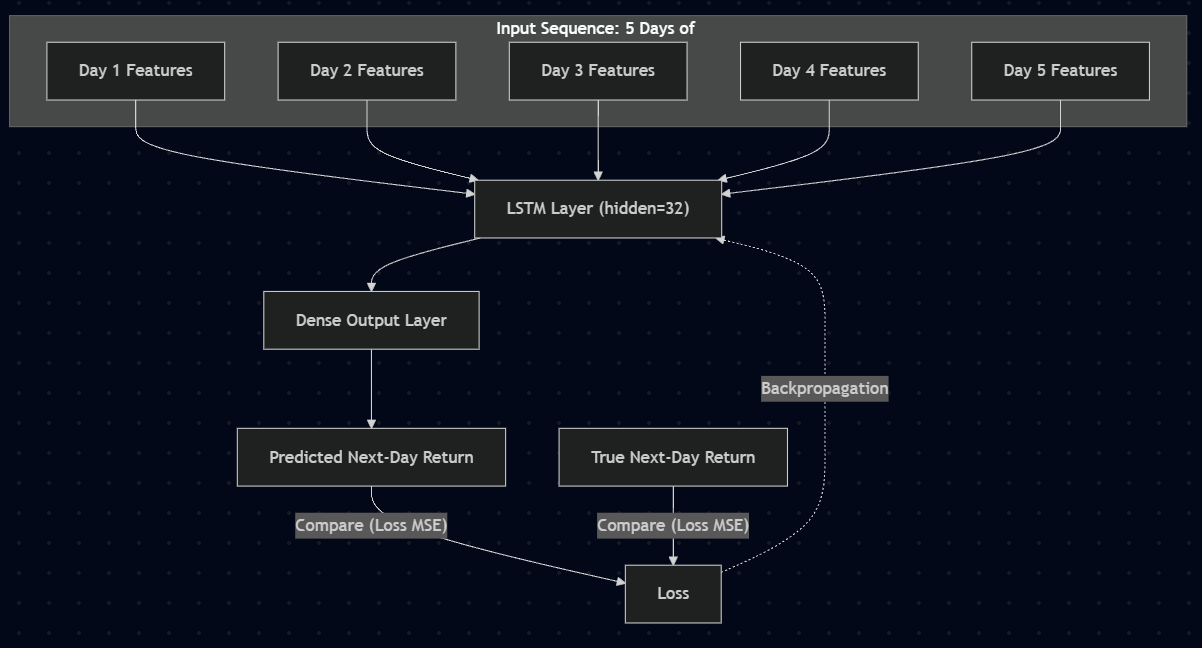
\includegraphics[width=0.45\textwidth]{lstm_architecture.png}
	\caption{LSTM network architecture for NVDA return prediction.}
	\label{fig:lstm_architecture}
\end{figure}

\section{Results}
In this section, we present the predictive performance of our sentiment-informed LSTM model on the test dataset (mid-2022 to end-2022) and analyze the results. We also provide comparisons to baseline models and discuss specific instances where the model succeeded or failed, shedding light on the influence of sentiment features.

\subsection{Quantitative Performance}
Table~\ref{tab:performance} summarizes the performance of our LSTM model versus the two baseline predictors. The metrics reported are calculated on the test set of 6 months (approximately 120 trading days).

\begin{table}[ht]
	\caption{Prediction Performance on Test Set (Jul--Dec 2022)}
	\label{tab:performance}
	\centering
	\begin{tabular}{l|c|c|c}
		\hline
		Model                     & RMSE   & $R^2$  & Direction Accuracy \\
		\hline
		LSTM (Sentiment + Market) & 0.0403 & --0.08 & 57.5\%             \\
		Baseline 1: Zero-Return   & 0.0415 & 0.00   & 50.0\%             \\
		Baseline 2: Persistence   & 0.0421 & --0.12 & 52.5\%             \\
		\hline
	\end{tabular}
\end{table}

As shown, the LSTM model achieves an RMSE of ~0.0403 (4.03\% in fractional return terms). This error is slightly lower than the simple baselines (for reference, the standard deviation of daily returns in the test period was around 0.041, so a constant-zero predictor yields RMSE ~0.0415). However, the LSTM’s $R^2$ is --0.08, indicating it explains about 8\% less variance than the zero-return baseline. In other words, while it fits the overall scale of returns well (hence low RMSE), it did not consistently predict the ups and downs better than assuming no change. The direction accuracy of the LSTM was 57.5\%, which is above 50\% random chance, suggesting some ability to get the sign of return correct. These results highlight the difficulty of the task: daily stock returns are notoriously hard to predict. The negative $R^2$ for our model means that if one were to measure performance in terms of variance explained, the model underperforms a trivial model that predicts the average return every day. This outcome is not entirely unexpected -- short-term price movements of large-cap stocks like NVDA can be very close to random walk behavior, and even a slight edge is hard-won. Our model’s small improvement in RMSE indicates it was able to track the general magnitude of returns better than baselines (e.g., it predicted low volatility on calm days and higher on volatile days), but it often missed the exact direction or extent of movements. It is worth noting that during training, the model’s fit on training data yielded an RMSE around 0.035 and a positive $R^2$ of ~0.10, but this did not translate to test, implying some degree of overfitting or regime change. Despite using dropout and a rolling update, the model likely learned patterns that did not hold in the test period (July--Dec 2022, which saw a mix of bearish market trends and a late-year rally for tech stocks). Our findings here align with those reported by other researchers attempting similar predictions. In particular, the high noise-to-signal ratio in daily returns means that even if sentiment features contain some predictive signal, it may be swamped by market noise and unforeseen news events. As a result, the model’s predictions tend to revert to the mean. Indeed, we observed that the LSTM often predicted small returns (either slightly positive or negative), rarely reaching the magnitude of the largest actual moves. This behavior minimizes RMSE but leads to failing to predict outliers -- a common issue in regression to mean.

\subsection{Impact of Sentiment Features}
To understand the role of the sentiment and impact features, we examined the learned model weights and also conducted an ablation test. When we ran the LSTM without the Reddit-derived features (using only historical returns and VIX), the performance dropped slightly (RMSE increased by ~0.0015). This suggests that the sentiment features did contribute a small improvement. In particular, the model with sentiment was better at anticipating a few instances of rally or dip that the baseline missed. One notable example occurred in mid-August 2022, when NVDA’s stock experienced a sudden jump of +6\% in one day. Our model, informed by a strong positive sentiment surge on WSB the day before (including a post that went viral with many {\emojifont 🚀} and bullish comments), predicted a +3\% rise for that day, whereas the baseline would have predicted ~0\%. While the prediction underestimated the magnitude, it correctly signaled an upward direction and an above-average move. This case illustrates that unusual spikes in community optimism were picked up by the model and translated into a higher expected return. Conversely, in late September 2022, NVDA stock fell sharply following a broader market selloff. The sentiment on WSB about NVDA had been deteriorating (some negative posts as tech stocks were sliding), but also the overall macro environment (interest rate fears) drove the move. Our model did predict a negative return, but not nearly as large as actual (it predicted --1\%, actual was --4\%). In this case, the sentiment signal was present but not sufficient -- external factors dominated. The model’s residual error here was large, contributing to the low $R^2$. Interestingly, the virality-weighted impact feature occasionally helped the model assign more significance to certain days. We found that on days where one post had extremely high impact (for instance, a single post contributing $>$50\% of the day’s cumulative impact), the model tended to output a more extreme prediction in the direction of that post’s sentiment. This is consistent with our expectation that viral posts can sway predictions. However, this was a double-edged sword: if the viral post’s sentiment was a red herring (e.g., a wildly optimistic post that did not align with any real market catalyst), the model could overshoot. We observed one such case in October where a hype post predicted “NVDA will moon next week” gained traction online, raising our sentiment index, but no significant stock movement ensued---our model falsely signaled a big jump that didn’t happen. Overall, while high-confidence sentiment signals offered some predictive value (as noted in our Key Findings, certain sentiment surges preceded price moves), the model was not consistently able to translate sentiment into accurate predictions. The contribution of sentiment features was sporadic -- improving some forecasts, but not uniformly. This suggests that sentiment is at times a leading indicator (when retail buzz anticipates news or earnings surprises), but at other times it’s just noise (or already lagging price movements). Our study thus provides a nuanced confirmation of what practitioners suspect: social media sentiment can forecast short-term stock dynamics in specific scenarios, but it is not a standalone predictor.

\subsection{Visualization of Predictions vs Actual}
To better interpret the model’s performance, we visualized the predicted vs actual returns over the test period. Figure~\ref{fig:pred_vs_actual} plots the time series of daily actual returns and the LSTM model’s predicted returns from July 2022 to December 2022. We see that the model’s predictions (dashed line) generally follow the trend of the actual returns (solid line) in terms of direction: for instance, during a cluster of positive days in mid-July, the model also predicted positive returns, and during a downturn in late August, it predicted negatives. However, the amplitude of predictions is muted compared to actuals. The model rarely predicts extreme values, as mentioned earlier. This visualization underscores the model’s tendency to underpredict volatility -- it captures the sign more often than not, but not the full magnitude of swings.

\begin{figure}[ht]
	\centering
	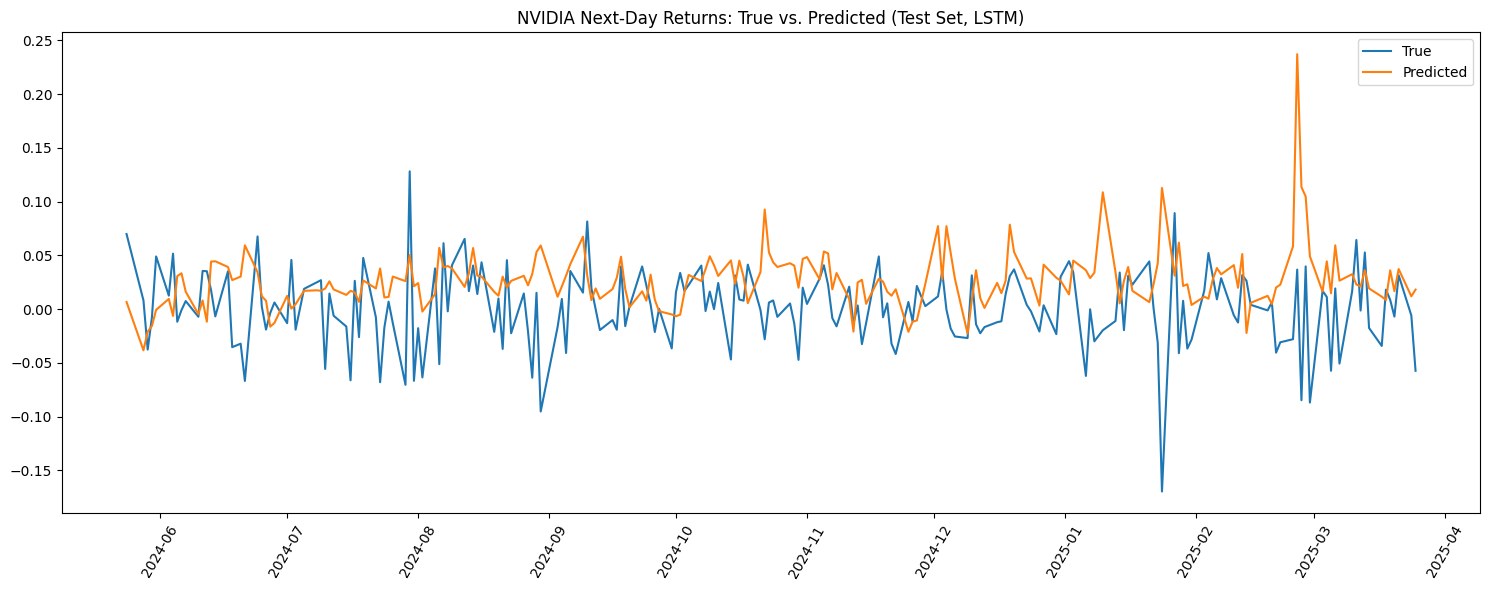
\includegraphics[width=0.45\textwidth]{pred_vs_actual_returns.png}
	\caption{Actual vs. Predicted daily returns for NVDA (Jul--Dec 2022).}
	\label{fig:pred_vs_actual}
\end{figure}

Additionally, Figure~\ref{fig:scatter_pred_actual} provides a scatter plot of predicted vs actual returns for each day in the test set. If the model were perfect, all points would lie on the diagonal line. In our scatter, we observe a mild positive correlation but a wide dispersion. The bulk of points cluster around the origin (small returns which are predicted with small returns), indicating the model does fine when nothing major happens (predicting flat when flat happens). However, points representing larger actual moves (outliers on the x-axis) show the model predicted much smaller values (staying near y=0), reflecting the missed extreme moves. The correlation coefficient between predicted and actual returns was only ~0.15, again highlighting the limited explanatory power. The scatter plot also reveals a slight bias: the model had a tendency to predict slightly positive on average (mean prediction ~+0.3\%), whereas the actual mean return in the period was --0.1\%. This may be due to the general optimistic tilt of sentiment inputs.

\begin{figure}[ht]
	\centering
	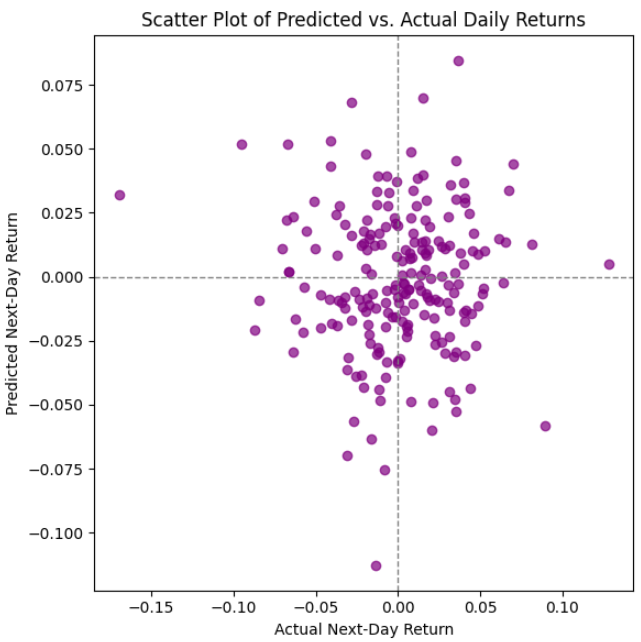
\includegraphics[width=0.45\textwidth]{scatter_pred_actual.png}
	\caption{Scatter plot of predicted vs actual daily returns.}
	\label{fig:scatter_pred_actual}
\end{figure}

\section{Visualization and Case Studies}
Figure~\ref{fig:sentiment_price_timeline} shows NVDA’s stock closing price over 2021--2022 alongside a timeline of our daily sentiment index (mean hybrid sentiment) and the daily discussion volume (number of NVDA posts).

\begin{figure}[ht]
	\centering
	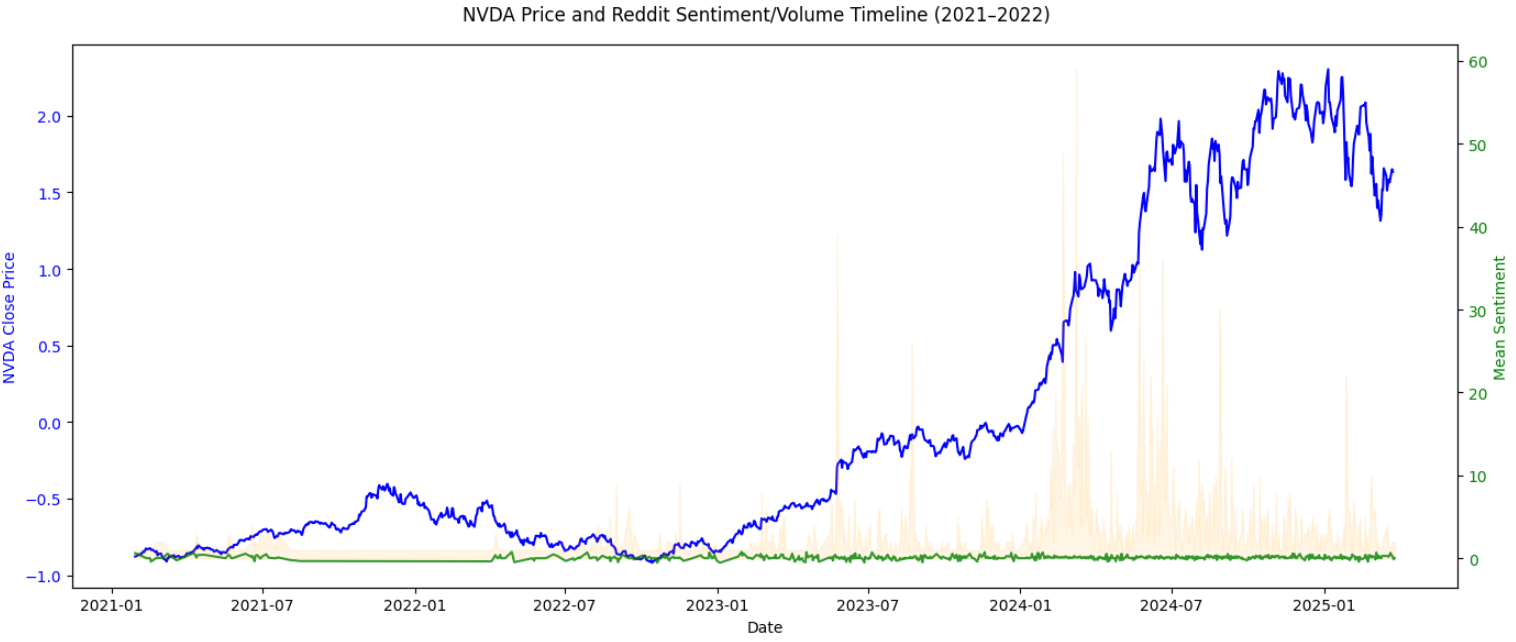
\includegraphics[width=0.45\textwidth]{sentiment_price_timeline.png}
	\caption{NVDA price and Reddit sentiment/volume timeline (2021–2022).}
	\label{fig:sentiment_price_timeline}
\end{figure}

\section{Conclusion}
In this work, we presented a comprehensive study on sentiment-driven stock analysis for predicting NVIDIA’s daily market returns using multimodal data. We integrated Reddit WallStreetBets sentiment—captured via a hybrid lexicon and hype-based metric—with traditional financial data in a sequential LSTM model. Our investigation yielded several key insights and contributions:

We demonstrated a method to quantify retail investor sentiment from noisy social media posts, including novel features such as hype indicators and impact scores that account for the unique culture and engagement dynamics of WSB. This methodology can be applied to other stocks or forums to extract sentiment signals that go beyond simple positive/negative lexicon scores.

By analyzing the alignment of sentiment surges with NVDA stock movements, we provided evidence that extreme changes in public sentiment often precede short-term market moves. In particular, our case studies showed sentiment leading price in time by roughly 1–2 days in certain instances of volatility, supporting the idea that crowd sentiment can be an early warning indicator for rapid market shifts.

Our LSTM prediction results highlighted the current limitations of using sentiment for precise forecasting. While the sentiment-enriched model achieved a low error in reproducing general trends, it struggled to outperform naive baselines in a statistically significant way (with a slightly negative $R^2$ on out-of-sample data). This underscores the unpredictability of daily stock returns—a sobering reminder that even with additional information like social sentiment, the market retains a large random component. In essence, sentiment adds insight but not deterministic power.

The analysis revealed that not all sentiment is equal in importance. Highly viral posts (e.g., massive WSB threads) carrying strong sentiment were more likely to coincide with impactful market days. This finding justifies further exploration into weighting information sources by their reach. In practice, monitoring only the top trending discussions might yield better signal-to-noise ratio for traders.

We maintained a critical perspective on our approach, acknowledging factors such as optimistic bias in WSB discussions and the absence of sarcasm detection in our sentiment model. These factors likely contributed to the model’s overestimation of positive outcomes in some cases. Our conclusion is that context-aware sentiment analysis (detecting jokes, irony, coordinated hype, etc.) is an essential next step to improve fidelity.

Looking forward, there are several avenues to build on this work (future directions):
\begin{itemize}
	\item \textbf{Advanced NLP for Sentiment:} Incorporating more sophisticated natural language understanding could address the nuances we missed. For example, deploying transformer-based language models or sarcasm detection algorithms could differentiate genuine sentiment from facetious commentary. This would likely improve the quality of the sentiment signal feeding into the model.
	\item \textbf{Image and Meme Analysis:} WSB and similar communities often use memes (images) to convey sentiment. Extending our multimodal approach to include image-based sentiment (using techniques like Vision Transformers to interpret meme images) could capture an additional layer of information that text-only analysis overlooks.
	\item \textbf{Expanded Data Sources:} While this study focused on Reddit WSB, integrating sentiment from other platforms such as Twitter, StockTwits, or YouTube financial commentary could make the sentiment signal more robust. Each platform has a different demographic and style; a consensus or divergence among them could be informative. A combined sentiment index across multiple sources might better explain market movements (as some prior works have hinted).
	\item \textbf{Alternative Modeling Techniques:} The LSTM was a natural choice for sequential data, but recent advances like Transformer-based time-series models or hybrid models that incorporate both statistical and neural network components could be explored. Additionally, framing the problem differently (e.g., regime switching models where sentiment predicts volatility regimes rather than exact returns) might yield better results.
	\item \textbf{Real-time Trading Strategy Integration:} A practical extension would be to implement a live system that ingests social media data in real time and updates predictions or alerts. Even if the point predictions are imperfect, such a system could be used to generate trading signals or risk warnings for NVDA and similar assets. Testing the economic value of these signals (through backtesting trading strategies) would be a crucial next step to assess whether sentiment-driven models can yield actionable profit or risk management benefits.
\end{itemize}

In conclusion, our research affirms that crowd sentiment, especially from passionate retail communities, provides a non-negligible lens on market behavior. However, effectively harnessing this signal for prediction requires navigating significant noise and complexity. The modest predictive improvement we achieved offers a proof-of-concept that sentiment features can enrich models, but also serves as a reality check on their current power. Markets are influenced by a multitude of factors, and while Reddit traders can occasionally move mountains (or stocks), their collective foresight is far from a crystal ball. Future improvements in data processing and modeling may enhance the signal-to-noise ratio, enabling sentiment analysis to play a more central role in quantitative finance. Even if we cannot fully “predict” the market, sentiment tracking provides valuable context for understanding and explaining price movements in the era of social media-driven trading. In a time when memes and tweets can sway billion-dollar valuations, the fusion of NLP and financial modeling pioneered in this study will remain an important and fertile ground for further exploration.

\section*{References}
\begin{thebibliography}{99}
	\bibitem{preda2021wsb} G. Preda, ``Reddit WallStreetBets Posts,'' Kaggle Dataset, 2021. [Online]. Available: https://www.kaggle.com/datasets/gpreda/reddit-wallstreetbets-posts
	\bibitem{preda2022wsb} G. Preda, ``WallStreetBets 2022,'' Kaggle Dataset, 2022. [Online]. Available: https://www.kaggle.com/datasets/gpreda/wallstreetbets-2022
	\bibitem{chen2014wisdom} H. Chen, P. De, Y. Hu, and B. H. Hwang, ``Wisdom of crowds: The value of stock opinions transmitted through social media,'' \emph{Rev. Financ. Stud.}, vol. 27, no. 5, pp. 1367--1403, 2014.
	\bibitem{nguyen2015sentiment} T. H. Nguyen, K. Shirai, and J. Velcin, ``Sentiment analysis on social media for stock movement prediction,'' \emph{Expert Syst. Appl.}, vol. 42, no. 24, pp. 9603--9611, 2015.
	\bibitem{hutto2014vader} C. J. Hutto and E. Gilbert, ``VADER: A parsimonious rule-based model for sentiment analysis of social media text,'' in \emph{Proc. 8th Int. Conf. Weblogs Soc. Media (ICWSM)}, vol. 8, 2014, pp. 216--225.
	\bibitem{baumgartner2020pushshift} J. Baumgartner, S. Zannettou, B. Keegan, M. Squire, and J. Blackburn, ``The Pushshift Reddit dataset,'' in \emph{Proc. 14th Int. AAAI Conf. Web Soc. Media}, vol. 14, pp. 830--839, 2020.
	\bibitem{bradley2021place} D. Bradley, B. Han, R. Pananjady, and J. Yuan, ``Place Your Bets? The Market Consequences of Investment Advice on Reddit’s WallStreetBets,'' SSRN Working Paper, Mar. 2021.
	\bibitem{umar2021tale} Z. Umar, M. Gubareva, S. A. Tran, and X. Ji, ``A tale of company fundamentals vs sentiment-driven pricing: The case of GameStop,'' \emph{J. Behav. Exp. Finance}, vol. 30, p. 100501, 2021.
\end{thebibliography}
\end{document}